\section{Results}

\subsection{Number of planets}
To investigate how the number of planets changes during a $5000$ years evolution of a solar system and how it varies with the parameter $N$(initial number of bodies). 
We varied $N$ from $100$ to $1000$ with step size $100$(thus $10$ different $N$'s). 
For each $N$, we ran $5$ simulations measured the average number of planets after every $10$ years. The following results are obtained:

\begin{figure}[H]
\centering
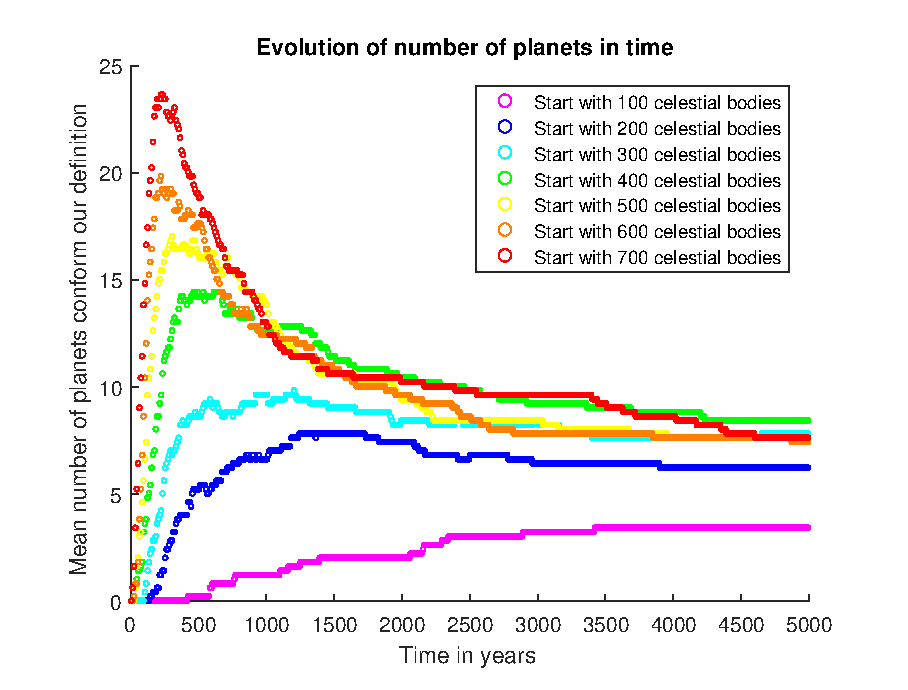
\includegraphics[scale=0.8]{AantPlaneten.eps}
\caption{Average number of planets during 5000 years of evolution, measured after each 10 years}
    \label{fig:AantPlaneten}
\end{figure}

As is shown in Figure \ref{fig:AantPlaneten}, planets are quickly formed in the early stadium of the evolution, and the more bodies there are, the more planets are formed in this stadium. 
This is logical, since the system is very dynamic in the early stadium due to the huge amount of bodies that gives rise to many collisions. 
After this early stadium, the small planets accrete further and become bigger planets, and the system becomes more and more stable until a sort of equilibrium is reached in which the number of planets is constant.\\

A remarkable result is that although a larger number of bodies at the start would result in a larger number of planets at the early stadium, the number of planets at the end is roughly the same independent of $N$, if $N$ is large enough(in our case around $N=300$). 
This should mean that a larger $N$ would only results in the formation of larger and heavier planets, which is confirmed in the next result:
\begin{figure}[H]
	\centering
	\begin{subfigure}{0.45\textwidth}
	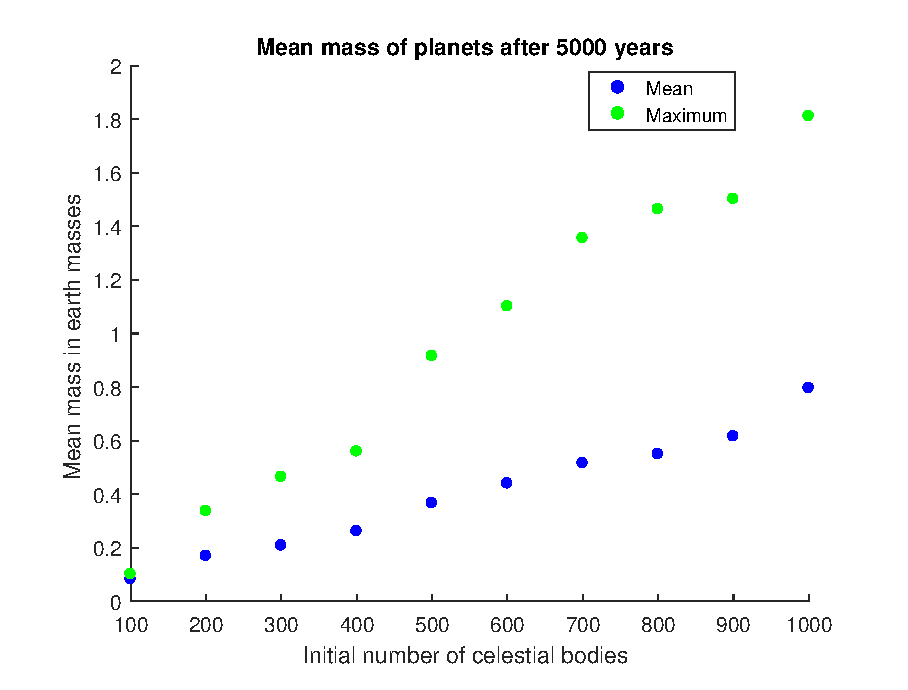
\includegraphics[width=\textwidth]{Eindmassa.eps}
	\caption{Average and maximal mass of planets after 5000 years.}
	\end{subfigure}
	~
	\begin{subfigure}{0.45\textwidth}
	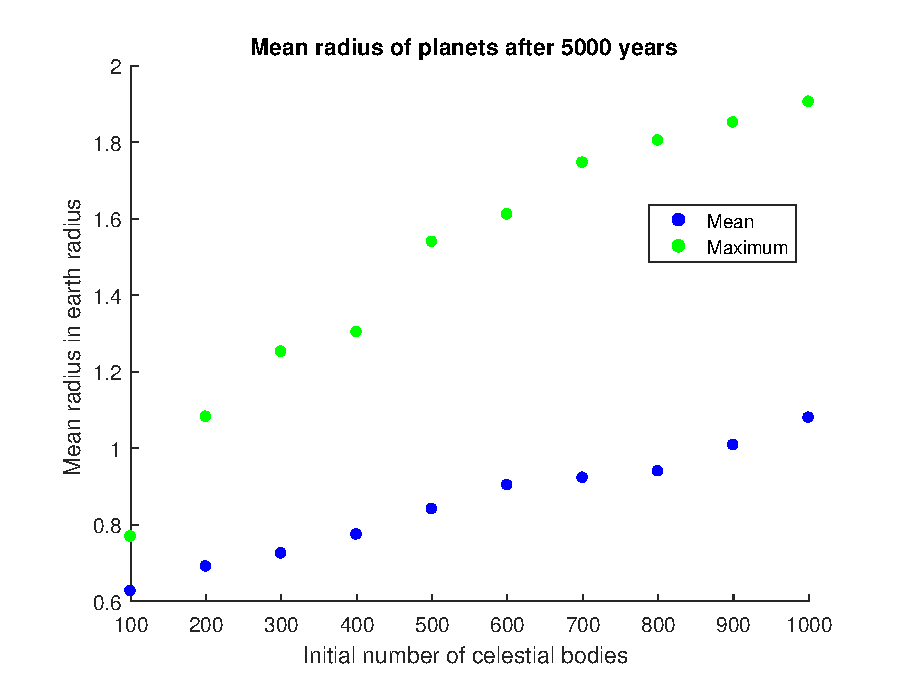
\includegraphics[width=\textwidth]{Eindstraal.eps}
	\caption{Average and maximal radius of planets after 5000 years.}
	\end{subfigure}
	\caption{The average and maximal mass and radius of planets after 5000 years, plotted against the number of initial bodies $N$. The average mass and radius of all planets in each one of the five simulations is first calculated, and then the average of the five averages was taken for each $N$.}
	\label{AverageMassandRadius}
\end{figure} 
Indeed, from figure \ref{AverageMassandRadius}, we see that on average larger and heavier planets are formed if $N$ is larger, which is very logical since the total mass in the system is conserved. And for the radius we have $\text{radius} \sim \sqrt[3]{\text{mass}}$, thus also greater radius is very logical. One interesting thing to note is that on average the heaviest planet we can get for $N=1000$ is of mass around $1.8M_{\oplus}$. If we assume that the maximal mass depends lineairly on $N$(which might not be a very bad approxmation by looking at figure \ref{AverageMassandRadius}, if we are only interested in the order of magnitude of $N$), then we would need about $334\cdot \frac{1000}{1.8}\approx 190000\sim 10^5$ bodies at the start to get Jupiter. 